\documentclass[../TV&MS.tex]{subfiles}
\begin{document}
    
\section{Виды сходимости случайных величин}

В этом разделе мы введем вагон непонятных определений, а потом постараемся запутаться еще больше, доказывая, какая сходимость круче, и ковыряясь в контрипримерах. Но для начала вспомним наших старых знакомых: измеримое пространство $(\Omega, \Ev)$, вероятностное пространство $(\Omega, \Ev, \Pro)$ и случайную величину $\xi \colon \Omega \rightarrow \Real$, которая обладает свойством
$$\forall B \in \Bor \quad \xi^{-1}(B) = \{ \omega \in \Omega \colon \xi(\omega) \in B \} \in \Ev$$

Пусть теперь $\xi, \xi_1, \xi_2, \dots$ "--- случайные величины на $(\Omega, \Ev)$.

\begin{Def}
Последовательность случайных величин $\{\xi_n\}$ \uline{сходится} к случайной величине $\xi$ \uline{почти наверное (с вероятностью 1)}, если вероятность множества тех элементарных событий, где она не сходится, равно нулю.
$$\{ \xi_n \} \xrightarrow{\text{п.н.}} \xi, \text{если} \quad \Pro(\Set{\omega}{\xi_n(\omega) \nrightarrow \xi}) = 0$$
\end{Def}

\begin{Ex}
Пусть $\xi_n$ принимает значение $n$ в рациональных точках числовой прямой и $0$ "--- в иррациональных. Тогда $\{\xi_n\} \xrightarrow{\text{п.н.}} 0$, так как мера множества рациональных чисел, где случайная величина расходится, "--- ноль.
\end{Ex}

\begin{Def}
Последовательность случайных величин $\{\xi_n\}$ \uline{сходится} к случайной величине $\xi$ \uline{в среднем порядка $r$}, если $r$-тый момент их разности сходится к нулю.
$$\{ \xi_n \} \xrightarrow{\text{(r)}} \xi, \text{если} \quad \Expec(\xi_n - \xi)^r \xrightarrow[n \rightarrow +\infty]{} 0$$
\end{Def}

\begin{Ex}
Возьмем в качестве множества $\Omega$ окружность длины 1, событиями будут борелевские множества, а вероятность введем как меру Лебега. События $A_n$ введем таким образом: $A_1$~"--- дуга длины $1/2$, отложенная от какой-то точки против часовой стрелки. $A_n$~"--- дуга длины $\frac{1}{n+1}$, отложенная против часовой стрелки от конца дуги $A_{n-1}$. Введем случайную величину: $\xi_n(\omega) = \Ind(\omega \in A_n)$
Покажем, что $\{\xi_n\}$ сходится к $0$ в среднем любого положительного порядка.
$$\Expec(\xi_n - \xi)^r = \Expec\xi_n^r = \Expec\left(\Ind(\omega \in A_n)\right)^r = \Pro(A_n) = 1/n \xrightarrow[n \rightarrow +\infty]{} 0$$
\end{Ex}

\begin{St}
Из сходимости в среднем, вообще говоря, не следует сходимость почти наверное.
\end{St}

\begin{Proof}
В рассмотренном выше примере $\xi_n(\omega)$ не сходится ни в одной точке окружности. Действительно, так как ряд $\sum_{n=1}^\infty \frac{1}{n}$ расходится, то для любой точки $\omega$ на окружности мы можем указать бесконечное число номеров $n_k$, таких что $\omega~\in~A_{n_k}$.~
\end{Proof}

\begin{St}
Из сходимости почти наверное, вообще говоря, не следует сходимость в среднем.
\end{St}

\begin{Proof}
Рассмотрим отрезок $[0, 1]$, с событиями, являющимися борелевскими множествами и вероятностью, введенной как мера Лебега. Положим $\xi_n(\omega) = e^{n} \Ind(\omega \in [0, 1/n])$. Тогда $\xi_n \xrightarrow{\text{п.н.}} 0$, но при этом $\forall r > 0 \quad \Expec\xi_n^r = e^{np}\Expec\Ind(\omega \in [0, 1/n]) = e^{np}/n$, а эта величина стремится к бесконечности, значит, сходимости в среднем нет.~
\end{Proof}

Введем еще один вид сходимости.

\begin{Def}
Последовательность случайных величин $\{\xi_n\}$ \uline{сходится} к случайной величине $\xi$ \uline{по вероятности}, если для любого сколь угодно малого положительного $\varepsilon$ вероятность таких событий, что модуль разности $\xi_n$ и $\xi$ больше $\varepsilon$, стремится к $0$.
$$\{\xi_n\} \xrightarrow{\Pro} \xi, \text{если} \quad \forall \varepsilon > 0 \quad \Pro(\Set{\omega}{|\xi_n(\omega) - \xi(\omega)| > \varepsilon}) \xrightarrow[n \rightarrow +\infty]{} 0$$
\end{Def}

\begin{Wtf}
На этом моменте может немного поплавиться мозг в попытках понять, чем сходимость по вероятности отличается от сходимости с вероятностью 1. Действительно, и там и там мы говорим, что вероятность тех событий, на которых случайная величина не сходится, равна нулю. Но разница в том, что в случае сходимости почти наверное мы сначала устремляем $n$ к бесконечности, а потом считаем вероятность, событий, когда не сходится, а в случае сходимости по вероятности мы сначала посчитали вероятность для какого-то фиксированного $n$, а потом устремились к бесконечности. 
\end{Wtf}

\begin{Ex}
Докажем, что та жуткая последовательность случайных величин на окружности сходится по вероятности к нулю. Действительно, 
$$\Pro(\Set{\omega}{|\xi_n(\omega) - 0| > \varepsilon}) = \Pro(\Set{\omega}{\xi_n(\omega) > \varepsilon}) = \Pro(\Set{\omega}{\xi_n(\omega) = 1}) = 1/n \xrightarrow[n \rightarrow +\infty]{} 0$$
\end{Ex}

\begin{St}
Только что рассмотренным примером мы доказали, что из сходимости по вероятности, вообще говоря, не следует сходимость почти наверное.
\end{St}

\begin{St}
Из сходимости по вероятности, вообще говоря, не следует сходимость в среднем.
\end{St}

\begin{Proof}
Для доказательства воспользуемся примером про отрезок. Докажем, что $\{\xi_n\} \xrightarrow{\Pro} 0$. Действительно, $\Pro{\Set{\omega}{\xi_n(\omega) > \varepsilon}} = 1/n \xrightarrow[n \rightarrow +\infty]{} 0$. Отсутствие сходимости в среднем мы уже доказали.
\end{Proof}

\begin{Th}
Из сходимости почти наверное следует сходимость по вероятности.
\end{Th}

\begin{Proof}
Сначала докажем, что $\{ \xi_n \} \xrightarrow{\text{п.н.}} \xi \quad \Leftrightarrow \quad \Pro\left(\sup \limits_{k \geqslant n} |\xi_k -\xi| \geqslant \varepsilon\right) \rightarrow 0$. Положим $A_n^\varepsilon = \Set{\omega}{|\xi_n -\xi| \geqslant \varepsilon}$, 
$A^\varepsilon = \varlimsup A_n^\varepsilon \equiv \bigcap\limits_{n=1}^\infty \bigcup\limits_{k \geqslant n} A_k^\varepsilon$. Тогда:
$$\Pro\left(\Set{\omega}{\xi_n(\omega) \nrightarrow \xi}\right) = 0 \quad \Leftrightarrow \quad \Pro\left(\bigcup_{\varepsilon > 0} A^\varepsilon\right) = 0 \quad \Leftrightarrow \quad \Pro\left(\bigcup_{m=1} A^{1/m}\right) = 0 \quad \Leftrightarrow$$
$$\Leftrightarrow \quad \Pro(A^{1/m}) = 0, m \geqslant 1 \quad \Leftrightarrow \quad \Pro(A^\varepsilon) = 0, \varepsilon > 0 \quad \Leftrightarrow \quad 
\Pro\left( \bigcup_{k \geqslant n} A_k^\varepsilon \right) \xrightarrow[n \rightarrow \infty]{} 0, \varepsilon > 0 \quad \Leftrightarrow$$
$$\Leftrightarrow \quad \Pro\left(\sup \limits_{k \geqslant n} |\xi_k -\xi| \geqslant \varepsilon\right) \xrightarrow[n \rightarrow \infty]{} 0 \quad \Rightarrow \quad \Pro\left( |\xi_k - \xi| \geqslant \varepsilon \right) \rightarrow 0.$$
А последнее утверждение "--- это определение сходимости по вероятности.
\end{Proof}

\begin{Wtf}
Совершенно жуткое доказательство, понимается методом вглядывания: если достаточно долго медитировать над каждой импликацией, то все переходы в конце концов станут понятными.
\end{Wtf}

\begin{Th}
Из сходимости в среднем следует сходимость по вероятности.
\end{Th}

\begin{Proof}
Утвеждение теоремы практически сразу же следует из обобщенного неравентва Чебышева:
$$\Pro \left( |\xi_n - \xi| \geqslant \varepsilon \right) \leqslant \frac{\Expec|\xi_n - \xi|^r}{\varepsilon^r}.$$
Переходя в неравенстве к пределу при $n \rightarrow \infty$, получаем требуемое.
\end{Proof}

\begin{Def}
Последовательность случайных величин $\{\xi_n\}$ \uline{слабо сходится} к случайной величине $\xi$, если для любой непрерывной и ограниченной функии последовательность мат. ожиданий функций от $\xi_n$ сходится к мат. ожиданию функции от $\xi$.
$$\{ \xi_n \} \xrightarrow{w} \xi, \text{если} \quad \forall f(x) \colon f(x) \in C \  \text{и} \  |f(x)| \leqslant M \quad \Expec{f(\xi_n)} \rightarrow \Expec{f(\xi)}$$
\end{Def}

\begin{St}
Из сходимости по вероятности следует слабая сходимость.
\end{St}

\begin{Proof}
Пусть $f(x) \colon |f(x)| \leqslant M.$ Также $\forall \varepsilon > 0$ выберем $N$ так, чтобы $\Pro{|\xi| > N} \leqslant \dfrac{\varepsilon}{4M}.$ Выберем $\delta$ так, чтобы $\forall |x| \leqslant N$ и $|x - y| \leqslant \delta$ было выполнено неравенство $|f(x) - f(y)| \leqslant \varepsilon/2$. Тогда:
\begin{multline*}
	\Expec{|f(\xi_n) - f(\xi)|} =
	\Expec{\left(|f(\xi_n) - f(\xi)|; |\xi_n - \xi| \leqslant \delta; |\xi| \leqslant N\right)} + \\
	\Expec{ \left( |f(\xi_n) - f(\xi)|; |\xi_n - \xi| \leqslant \delta; |\xi| > N \right) } +
	\Expec{ \left( |f(\xi_n) - f(\xi)|; |\xi_n - \xi| > \delta) \right) } \leqslant \\
	\varepsilon/2 + \varepsilon/2 + 2M * \Pro(|\xi_n - \xi| > \delta) = \varepsilon + \Pro(|\xi_n - \xi| > \delta).
\end{multline*}
Но из сходимости по веротности следует, что $\Pro(|\xi_n - \xi| > \delta) \rightarrow 0$, значит при $n~\rightarrow~\infty \qquad \Pro(|\xi_n - \xi| > \delta) < \varepsilon$, тогда $\Expec{|f(\xi_n) - f(\xi)|} < 2\varepsilon$, откуда в силу произвольного выбора $\varepsilon$ и в силу того, что модуль числа не превосходит самого числа, получаем требуемое.
\end{Proof}


\begin{Def}
Последовательность слeчайных величин $\{\xi_n\}$ \uline{сходится} к случайной величине $\xi$ \uline{по распределению}, если функции распределения $\{\xi_n\}$ сходятся к функции распределения $\xi$ во всех точках, в которых предельная функция распределения непрерывна.
$$\{ \xi_n \} \xrightarrow{d} \xi, \text{если} \quad F_{\xi_n}(x) \rightarrow F_\xi \quad \forall x \colon F_\xi(x) \in C(x)$$
\end{Def}

\begin{Ex}
Пусть $\{ \xi_n \}$ принимает значения $0$ и $1 - \dfrac{1}{n}$ с вероятностями $\dfrac{1}{2}$. Тогда функция распределения для случайной величины $\xi_i$ выглядит так (Рис.~\ref{ris:distr_seq}): 
\\
\begin{minipage}{0.32\linewidth}
	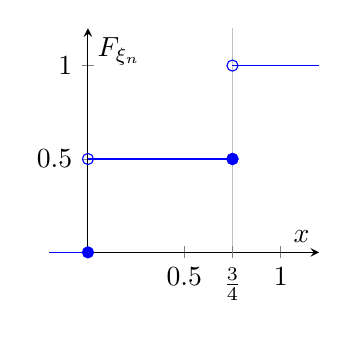
\begin{tikzpicture}
	\begin{axis}[
		scale=0.5,
		axis x line = middle,
		axis y line = middle,
		xlabel = {$x$},
		ylabel = {$F_{\xi_n}$},
		domain=-0.2:1.2
		ymin=-0.2,
		ymax=1.2,
		extra x ticks={0.75},
		extra x tick style={
			grid=major
		},
		extra x tick label={$\frac{3}{4}$}
	]
	\addplot[blue, domain=-0.2:0] {0};
	\addplot[blue, mark=*] coordinates {(0, 0)};
	\addplot[blue, mark=o] coordinates {
		(0, 0.5)
		(0.75, 0.5)
	};
	\addplot[blue, mark=*] coordinates {(0.75, 0.5)};
	\addplot[blue, mark=none, domain=0.75:1.2] {1};
	\addplot[blue, mark=o] coordinates {(0.75, 1)};
	\end{axis}
	\end{tikzpicture}
	\captionof{figure}{Функция распределения $\xi_n$ при $n = 4$}
	\label{ris:distr_seq}
\end{minipage}
\hfill
\begin{minipage}{0.32\linewidth}
	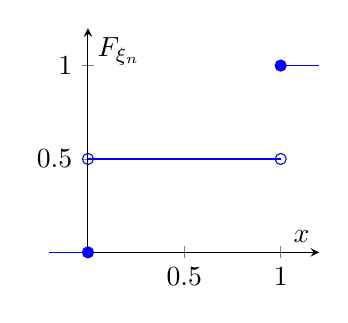
\begin{tikzpicture}
	\begin{axis}[
		scale=0.5,
		axis x line = middle,
		axis y line = middle,
		xlabel = {$x$},
		ylabel = {$F_{\xi_n}$},
		domain=-0.2:1.2
		ymin=-0.2,
		ymax=1.2
	]
	\addplot[blue, domain=-0.2:0] {0};
	\addplot[blue, mark=*] coordinates {(0, 0)};
	\addplot[blue, mark=o] coordinates {
		(0, 0.5)
		(1, 0.5)
	};
	\addplot[blue, mark=none, domain=1:1.2] {1};
	\addplot[blue, mark=*] coordinates {(1, 1)};
	\end{axis}
	\end{tikzpicture}
	\captionof{figure}{Предельная функция}
	\label{ris:limit_f}
\end{minipage}
\hfill
\begin{minipage}{0.32\linewidth}
	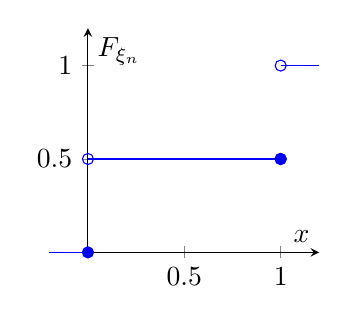
\begin{tikzpicture}
	\begin{axis}[
		scale=0.5,
		axis x line = middle,
		axis y line = middle,
		xlabel = {$x$},
		ylabel = {$F_{\xi_n}$},
		domain=-0.2:1.2
		ymin=-0.2,
		ymax=1.2
	]
	\addplot[blue, domain=-0.2:0] {0};
	\addplot[blue, mark=*] coordinates {(0, 0)};
	\addplot[blue, mark=o] coordinates {
		(0, 0.5)
		(1, 0.5)
	};
	\addplot[blue, mark=*] coordinates {(1, 0.5)};
	\addplot[blue, mark=none, domain=1:1.2] {1};
	\addplot[blue, mark=o] coordinates {(1, 1)};
	\end{axis}
\end{tikzpicture}
\captionof{figure}{Функция распределения $\xi$}
\label{ris:dist_lim}
\end{minipage}
\par\bigskip
Тогда предельная функция будет выглядеть так (Рис.~\ref{ris:limit_f}). Заметим, что она вообще не является функцией распределения, так как в точке $1$ нарушено условие непрерывности слева. Тогда рассмотрим случайную величину $\xi$, принимающую значение $0$ и $1$ с вероятностями $1/2$, тогда ее функция распределения имеет вид (Рис.~\ref{ris:dist_lim}). Заметим, что предельная функция и функция распределения $\xi$ различаются только в точке $1$, в которой $F_\xi(x)$ не является непрерывной, значит $\{\xi_n\} \xrightarrow[]{d} \xi.$
\end{Ex}

\begin{St}
Сходимость по распределению эквивалентна слабой сходимости.
\end{St}

\begin{Proof}
\uline{\textbf{TODO:}} Чет я не знаю, как это доказать =(
\end{Proof}

\begin{St}
Если последовательность случайных величин $\{ \xi_n \}$ сходится по распределению к вырожденной случайной величине $\xi \xequiv{\text{п.н.}} a$, то $\{ \xi_n \}$ сходится к $\xi$ по вероятности.
\end{St}

\begin{Proof}
Ы
\end{Proof}

А теперь докажем теорему, ради которой мы и городили все эти огороды сходимостей. Эта теорема впоследствии будет использоваться при доказательстве центральной предельной теоремы.

\begin{Th}[теорема Леви о непрерывности]
~\\
\begin{enumerate}
	\item Пусть $\{ \xi_n \} \xrightarrow{d} \xi$ \ и \ $f_n(t) := \Expec e^{it\xi_n}$.\ Тогда $\{ f_n(t) \} \rightarrow f(t)$,\ где $f(t) = \Expec e^{it\xi}$.
	\item Пусть теперь $f_n(t) := \Expec e^{it\xi_n}$. Тогда если $f_n(t) \rightarrow f(t) \quad \forall t \in \Real, \quad f(t) \in C(0)$, то $f(t)$ является характеристической функцией некоторой случайной величины $\xi$, такой что $\{ \xi_n \} \xrightarrow{d} \xi.$ 
\end{enumerate}
\end{Th}

\begin{Proof}
\begin{enumerate}
	\item Как было показано выше, сходимость по распределению эквивалентна слабой сходимости. Положим в определении слабой сходимость функции $\phi(x) := Re(e^{itx})$ и $\psi(x) := Im(e^{itx})$, тогда $\Expec\phi(\xi_n) \rightarrow \Expec\phi(\xi)$ и $\Expec\psi(\xi_n) \rightarrow \Expec\psi(\xi)$, откуда следует утверждение теоремы.
	\item Достаточно грустное доказательство, но, если у меня будет настроение, я его напишу. 
\end{enumerate}
\end{Proof}

\begin{Wtf}
А вот картинка, на которой схематично показано, что из чего следует.
\end{Wtf}

\begin{center}
\begin{tikzpicture}
	[
		st/.style={rectangle,draw}
	]
	\node[st] (prob1) {$\{ \xi_n \} \xrightarrow{\text{п.н.}} \xi$};
	\node[rectangle] (empty) [below=of prob1] {~};
	\node[st] (power) [below=of empty] {$\{ \xi_n \} \xrightarrow{(r)} \xi$};
	\node[st] (pro) [right=of empty] {$\{ \xi_n \} \xrightarrow{(\Pro)} \xi$};
	\node[st] (distr) [right=of pro] {$\{ \xi_n \} \xrightarrow{(d)} \xi$};
	\node[st] (weak) [below=of distr] {$\{ \xi_n \} \xrightarrow{(w)} \xi$};	
	\node (pn) at (3.8, -0.2) {$\xi \xequiv{\text{п.н.}} a$};
	\node[st] (th) [right=of distr] {т. о непрерывности};
	
	\draw [->] (prob1) -> (pro);
	\draw [->] (power) -> (pro);
	\draw [->] (pro) -> (distr);
	\draw [<->] (distr) -> (weak);
	\draw [->] (distr) to[bend right=45] (pro);
	\draw [dotted, line width=2pt] (distr) -> (th);
\end{tikzpicture}
\end{center}

\newpage



\end{document}
